% document formatting
\documentclass[10pt]{article}
\usepackage[utf8]{inputenc}
\usepackage[left=1in,right=1in,top=1in,bottom=1in]{geometry}
\usepackage[T1]{fontenc}
\usepackage{xcolor}

% math symbols, etc.
\usepackage{amsmath, amsfonts, amssymb, amsthm}

% lists
\usepackage{enumerate}

% images
\usepackage{graphicx} % for images

% code blocks
\usepackage{minted, listings} 

% verbatim greek
\usepackage{alphabeta}

\graphicspath{{./assets/images}}

\newcommand{\solution}{\textbf{Solution:}} 
\newcommand{\example}{\textbf{Example: }}
\newcommand{\R}{\mathbb{R}}

\title{BIOMATH 208 Week 6}

\author{Aidan Jan}
\date{\today}

\begin{document}
\maketitle

\section*{Review}
Groups are a practical example of manifold data we encounter a lot
\begin{itemize}
    \item e.g., rotation matrices, and other types of invertible matrix functions.
    \item Axioms are a relaxation of $+$ in a vector space.  We need a set $G$ and a binary operation $\circ\::\: G \times G \rightarrow G$ that satisfy three axioms:
    \begin{enumerate}
        \item Associative
        \item Neutral Element
        \item Inverse Element
    \end{enumerate}
\end{itemize}
There are a few subsets of groups:
\begin{itemize}
    \item Discrete groups: $\circ$ can be written with a Cayley table (always can write a Cayley table if the group is finite, which is most of the time)
    \item Lie group: Elements can be represented as a smooth manifold, and $\circ$, $^{-1}$ functions need to be smooth functions of the parameters
    \item Matrix groups are an important example of Lie groups.
    \begin{itemize}
        \item GL group (invertible $N \times N$ matrices)
        \item Affine transformation group (homogeneous coordinates), e.g., linear transformations and translations
    \end{itemize}
\end{itemize}
Use group actions in imaging:
\begin{itemize}
    \item affine matrix acting on points  $Ax$
    \begin{itemize}
        \item $(d + 1) \times N$ matrix of $N$ points in $d$ dimensions in homogeneous cooridnates
    \end{itemize}
    \item on normal vectors
    \begin{itemize}
        \item $A^{-T} n$
    \end{itemize}
    \item on images
    \begin{itemize}
        \item $(A \cdot I)(x) = I(A^{-1}x)$
        \item If images are discrete, we will discretize them again after transforming, this is not a group action.
    \end{itemize}
\end{itemize}

\section*{Tangent Spaces}
We want to build up a tool to understand differentiation on manifolds.  This will enable us to do gradient based optimization (e.g., gradient descent), and understand rates of change of various quantities.\\\\
We will approach this by considering parameterized curves ($\mathbb{R} \rightarrow \mathcal{M}$), and consider how functions ($\mathcal{M} \rightarrow \mathcal{R}$) change with respect to the curve's velocity.

\subsection*{What is Velocity?}
We typically define velocity as "change in position over time". which fundamentally depends on choice of a chart.  Here, we will use a different description, based only on curves.

\subsection*{Parameterized Curves}
Consider $(a, b) \in \mathbb{R}$ and a curve $\gamma \::\: (a, b) \rightarrow \mathcal{M}$.  Assume $0 \in (a, b)$ and let $\gamma(0) = p$ for some $p \in \mathcal{M}$.
\begin{itemize}
    \item $\gamma$ is a function with domain $\mathbb{R}$ and range $\mathcal{M}$.
\end{itemize}

\subsection*{Definition: Velocity of a Curve}
Let $f$ be some smooth function from $\mathcal{M} \rightarrow \mathbb{R}$ ($f \in \mathbb{C}^\infty (\mathcal{M})$).  Then the velocity of the curve is a map
\[v_{\gamma, p} \::\: \mathbb{C}^\infty \rightarrow \mathbb{R}\]
defined by
\[v_{\gamma, p} (f) = \frac{\text{d}}{\text{d}t} f \circ \gamma(t) \bigg|_{t = 0}\]
Note the right side is just a map from $\R \rightarrow \R$, so we can use standard calculus here.

\subsection*{Velocities are linear maps}
Based on the above definition, these maps are linear.  To prove this, we need to show that they are compatible with $+$ and $\cdot$.
\subsubsection*{Proof}
Let $f, g \in \mathbb{C}^\infty$ and $c \in \R$.  Then,
\begin{align*}
    v_{\gamma, p}(f + g) &= \frac{\text{d}}{\text{d}t} (f + g)(\gamma(t)) \bigg|_{t = 0}\\
    &= \frac{\text{d}}{\text{d}t} f(\gamma(t)) + g(\gamma(t)) \bigg|_{t = 0}\\
    &= \frac{\text{d}}{\text{d}t} f(\gamma(t)) \bigg|_{t = 0} + \frac{\text{d}}{\text{d}t}  g(\gamma(t)) \bigg|_{t = 0}\\
    &= v_{\gamma, p}(f) + v_{\gamma, p}(g)
\end{align*}
and,
\begin{align*}
    v_{\gamma, p}(cf) &= \frac{\text{d}}{\text{d}t} (c \cdot f)(\gamma(t)) \bigg|_{t = 0}\\
    &= \frac{\text{d}}{\text{c}} c \cdot_{\R} f(\gamma(t)) \bigg|_{t = 0}\\
    &= c \cdot v_{\gamma, p}(f)
\end{align*}

\subsection*{The Tangent Space to $\mathcal{M}$ at the point $p$}
\begin{center}
    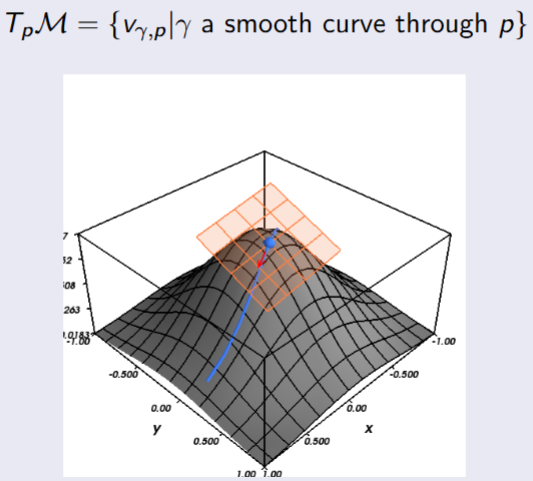
\includegraphics[width=0.8\textwidth]{W6_1.png}
\end{center}
\begin{itemize}
    \item Note that there are an infinite number of curves that pass through $p$.
    \item If we want to check if a linear map is a velocity, we need to find which curve it corresponds to.
    \item On a smooth manifold, every line passing through $p$ has the same velocity!
    \item $\mathcal{M}$ is a curved surface.  The orange plane, where all the tangents passing through $p$, is referred to as the \textbf{tangent plane}.
    \item The tangent plane is orthogonal to the normal vector at $p$.
\end{itemize}

\subsubsection*{The Tangent Space is a Vector Space}
\textbf{Definition: Addition of Velocities}\\\\
We define $(v_{\alpha, p} + v_{\beta, p})(f) = v_{\alpha, p}(f) + v_{\beta, p}(f)$.  We must show there is a curve in $T_p \mathcal{M}$ corresponding to the left side.\\\\
\textbf{Proof:}  We chose some chart $U, x$, with $p \in U$ and assume (without loss of generality) $x(p) = 0$.  Then consider
\[\gamma(t) = x^{-1}(x(\alpha(t)) + x(\beta(t)))\]
\begin{itemize}
    \item $p$ is in the coordinate neighborhood, $U$.
\end{itemize}
\textbf{Proof:}
Let's show it has the correct action:
\begin{align*}
    v_{\gamma, p} (f) = \frac{\text{d}}{\text{d}t} f(\alpha(t)) \bigg|_{t = 0} \\
    &= \frac{\text{d}}{\text{d}t} f(x^{-1}(x(\alpha(t)) +_{\mathbb{R}^+}) x(\beta(t)))\bigg|_{t = 0}\\
    \intertext{Look at $f \circ x^{-1}\::\: \R^3 \rightarrow \R$, $x \cdot \alpha$ or $x \cdot \beta \::\: \R \rightarrow \R^d$}
    [FILL]
\end{align*}

\textbf{Definition: Scalar Multiplication of Velocities}\\\\
We define scalar multiplication by changing the speed we move along a curve.  For $c \in \R$, let $\beta(t) = \gamma(ct)$.  Then,
\begin{align*}
    (c \cdot v{\gamma, p})(f) &= c \cdot v_{\gamma, p}(f)\\
    &= \frac{\text{d}}{\text{d}t} f(\gamma(ct)) \bigg|_{t = 0} = c \frac{\text{d}}{\text{d}t} f()
    [FILL]
\end{align*}

\subsection*{Action of a velocity in a chart}
Let's evaluate the action of a velocity $v$ on a function $f$ in a coordinate neighborhood ($U, x$).  With $p \in U, \gamma(0) = p$, and $x(p) = 0$.
\begin{itemize}
    \item $T, \mathcal{M}$ should have the same dimension and some basis (assuming dimension is finite).
\end{itemize}
\begin{align*}
    v_{\gamma, p}(f) &= \frac{\text{d}}{\text{d}t}f \cdot \gamma(t) \bigg|_{t = 0} \\
    &= \frac{\text{d}}{\text{d}t} f \circ x^{-1} \circ x \circ \delta(t) \bigg|_{t = 0}\\
    \intertext{Note that $\gamma \::\: \R \rightarrow \mathcal{M}$, $x \::\: \mathcal{M} \rightarrow \R^d$, $x^{-1} \::\: R^d \rightarrow \mathcal{M}$, $f \::\: \mathcal{M} \rightarrow \R$}
    &= \frac{\text{d}}{\text{d}t} (f \circ x^{-1}) \circ (x \circ \gamma)(0) \\
    &= [(f \circ x^{-1}) \circ (x \circ \gamma)]'(0)\\
    &= \partial_i (f \circ x^{-1})(x(p)) \cdot [(x \cdot \gamma)^i]'(0)
\end{align*}
\subsubsection*{A More Familiar Notation}
We rewrite the first term as:
\[\partial_i(f \circ x^{-1})(x(p)) \doteq \left(\frac{\text{d}f}{\text{d}x^i}\right)_p = \left(\frac{\partial}{\partial x^i}\right)_p(f)\]
We rewrite the second term as
\[[(x \circ \gamma)^i]'(0) \doteq \dot{\gamma}_x^i(0)\]
\begin{itemize}
    \item The dot above the $\dot{\gamma}$ means "derivative with respect to time"
\end{itemize}
[FILL]

\subsection*{Identifying Components}
We can rewrite the above action as
\[v_{\gamma, p}(f) = \dot{\gamma_x}(0) \left(\frac{\partial}{\partial x^i}\right)(f)\]
or just the linear operator as
\[v_{\gamma, p} = \dot{\gamma_x}(0) \left(\frac{\partial}{\partial x^i}\right)\]
Unlike $\partial_i$, the notation $\frac{\partial}{\partial x^i}$ reminds us we are using the chart $x$.  Previously in vector calculus we would say "the directional derivative is the gradient dot the direction"

\subsection*{Chart Induced Basis}
The operators $\frac{\partial}{\partial x^i}$ form a basis of $T_p \mathcal{M}$ for $p \in U$.  If the dimension of $\mathcal{M}$ is $d$, there are $d$ basis elements in this $d$ dimensional vector space.
\subsubsection*{Proof}
We already showed that these vectors span the vector space, so we must show these vectors are linearly independent, i.e., show that
\[0 = \lambda^i \left(\frac{\partial}{\partial x^i}\right)_p \Longrightarrow \lambda^i = 0 \forall i\]
Let's do that:
\begin{align*}
    0 &= \lambda^i \left(\frac{\partial}{\partial x^i}\right)_p x^j\\
    \intertext{By definition of the partial derivative symbol, we get the following:}\\
    &= \lambda \partial_i (x^j \circ x^{-1})(x(p))
    \intertext{This essentially means, "what is the derivative of the $j$-th component with respect to the $i$-th component?"}
    &= \lambda^i \delta_i^j\\
    &= \lambda^j
\end{align*}
If we compare the left hand side with the right hand side, it implies that $\lambda^i = 0$.  Therefore, we have a $d$ dimensional vector space.

\subsection*{Chart Induced Change of Components}
Let $X \in T_p \mathcal{M}$ and let $(U, x)$ and $(V, y)$ be two charts with $p \in U \cap V$.  We can express this vector in either chart
\[X_{(y)}^i \left(\frac{\partial}{\partial y^i}\right) = X = X_{(x)}^i \left(\frac{\partial}{\partial x^i}\right)_p\]
These are related by
\[X_{(y)}^i = \left(\frac{\partial y^i}{\partial x^j}\right)_p x_{(x)}^j\]
\begin{itemize}
    \item $\partial x^j$ is the "down index"
    \item The entire fraction (coefficient of $X_{(x)}^j$) is a Jacobian matrix of chart transition map.
    \item A Jacobian is a non-linear map of linear maps.
\end{itemize}

\subsubsection*{Proof}
Consider acting on a smooth function $f$.
\begin{align*}
    \left(\frac{\partial}{\partial x^i}\right)_p f &= \partial_i (f \circ x^{-1})(x(p))\\
    \intertext{Now we will insert the identity $y^{-1}\circ y$}
    &= \partial_i[(f \circ y^{-1}) \circ (y \circ x^{-1})] (x(p))\\
    \intertext{Notice that $(y \circ x^{-1})$ is a chart transition map.  Applying the chain rule\dots}
    &= \partial_j (f \circ y^{-1})(y(p)) \cdot \partial_i (y \circ x^{-1})^j (x(p))\\
    &= \left(\frac{\partial y^j}{\partial x^i}\right)_p \left(\frac{\partial}{\partial y^j}\right)_p\\
    \intertext{Now, we plug this result into the original expression:}
    &= X_{(y)}^i \cdot \left(\frac{\partial}{\partial y^i}\right)_p = X = X_{(x)}^i \left(\frac{\partial y^j}{\partial x^i}\right)_p \left( \frac{\partial}{\partial y^j}\right)_p
\end{align*}
This quantity is multiplying the basis vector.  Therefore, these are the components in the new basis
\begin{itemize}
    \item Essentially, components in chart (y) (left hand side) is equal to the components in chart (x) times the Jacobian matrix (right hand side)
\end{itemize}

\subsubsection*{Example: Vectors in Cartesian and Polar Coordinates}
\begin{itemize}
    \item Consider the manifold $\mathcal{M} = \mathbb{R}^2$, with a standard topology and atlas smoothly compatible with the identity chart.  Let ($\mathbb{R}^2$, x) be the identity chart and ($V, y$) the polar chart where $V$ has the nonpositive $x$ axis cut out.
    \item Given a vector with components $X_{(x)}^i$ in chart $x$, we will find its components in chart $y$ and vice versa.
    \item To do so, we need to evaluate the Jacobian matrix of the chart transition map:
\end{itemize}
\[\left(\frac{\partial y^i}{\partial x^j}\right)_p = \partial_j (y^i \circ x^{-1})(x(p))\]
We derived $y \circ x^{-1} = (r, \text{sign}(x^1) \arccos(x^0 / r))$, where $r = \sqrt{(x^0)^2 + (x^1)^2}$.  We can use some identities,
\begin{align*}
    \partial_i r(x^0, x^1) &= \frac{x^i}{r(x^0, x^1)}\\
    \partial_i \frac{x^j}{r} &= \frac{\delta_i^j r^2 - x^j x^i}{r^3}\\
    \arccos'(t) = -\frac{1}{\sqrt{1 - t^2}}
\end{align*}
and compute
\[\partial_j y^i \circ x^{-1}(x(p)) = \begin{pmatrix} \frac{x^0}{r} & \frac{x^1}{r} \\ \frac{-x^1}{r^2} & \frac{x^0}{r^2} \end{pmatrix}\]
Consider a straight line in chart $x \::\: \gamma(t) = (t, t + 1)$, for $t \in (-1, 1)$.  In chart $y$, the curve takes the form
\[y \circ \gamma(t) = \left(\sqrt{t^2 + (t + 1)^2}, \text{sign}(t + 1) \arccos \left(\frac{t}{\sqrt{t^2 + (1 + t)^2}}\right)\right)\]
and the components of its tangent vectors take the form
\[\dot{\gamma_y} = \begin{pmatrix} \frac{x^0}{r} & \frac{x^1}{r} \\ \frac{-x^1}{r^2} & \frac{x^0}{r^2} \end{pmatrix} \begin{pmatrix} 1 \\ 1 \end{pmatrix} = \begin{pmatrix} \frac{x^0 + x^1}{r} \\ \frac{-x^1 + x^0}{r^2} \end{pmatrix}\]
If we graph the two charts, we get:
\begin{center}
    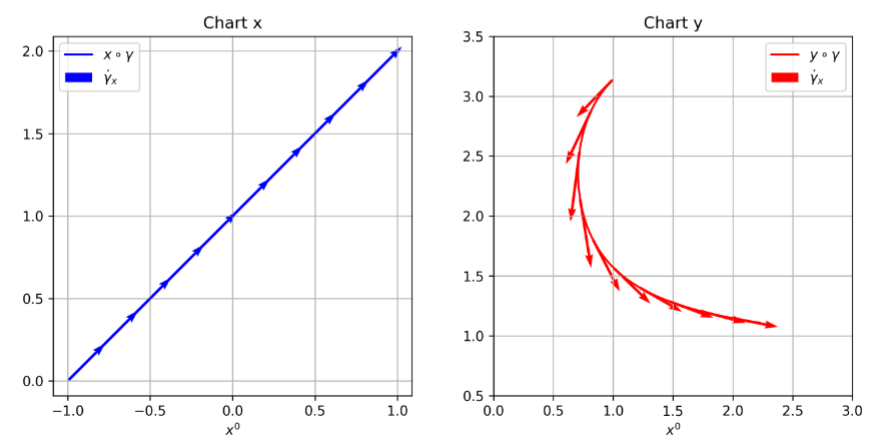
\includegraphics[width=\textwidth]{W6_2.png}
\end{center}
This shows that whether a line is straight or not depends on the choice of chart.

\subsection*{Push Forward of Vectors}
Consider two manifolds $\mathcal{M}$ and $\mathcal{N}$, and a smooth map $\phi \::\: \mathcal{M} \rightarrow \mathcal{N}$.  Let $f$ be a smooth function on $\mathcal{N}$.\\\\
If $X \in T_p \mathcal{M}$, we denote its push forward to $T_{\phi(p)}\mathcal{N}$ by $\phi_*(p)X \doteq \text{d} \phi (p)X$\\\\
It is defined by ites action on a function $(\phi_*(p)X)f = X(f \circ \phi)$.
\begin{itemize}
    \item $\text{d}\phi$ is the derivative of $\phi$, or the Jacobian of the function.
\end{itemize}

\subsection*{Push Forward in Local Coordinates}
Consider $\mathcal{M}$ with a chart $(U, x)$ and $\mathcal{Y}$ with a chart $(V, y)$.  Let $p \in U$ and $\text{d}\phi(p) \in V$.  Consider $X \in T_p \mathcal{M}$ given by $X = X^i \frac{\partial}{\partial x^i}$.  The coordinates of $\phi_*(p)X$ in the chart $y$ are given by
\[(\phi_*(p)X)_{(y)}^j = \left(\frac{\partial y^j \circ \phi}{\partial x^i}\right)_p X^i_{(x)}\]
That is, we multiply by the Jacobian matrix of the map $\phi$ in local coordinates.

\subsubsection*{Proof.}
Act on a function $f$ and start with the definition
\[(\phi_* (p)X)(f) = X(f \circ \phi)\]
Solving,
\begin{align*}
    &= X_{(x)}^i \left(\frac{\partial}{\partial x}\right)_p f \cdot \phi\\
    \intertext{By the definition of the partial derivative,}
    &= X_{(x)}^i \partial_i (f \circ \phi \circ x^{-1})(x(p))
    \intertext{Now, insert the identity map $y^{-1} \circ y$ and use the chain rule.}
    &= X_{(x)}^i \partial_i \left((f \circ y^{-1}) \circ (y \circ \phi \circ x^{-1})\right)(x(p))\\
    &= X_{(x)}^i \partial_j (f \circ y^{-1}) \bigg|_{y \circ \phi \circ x^{-1} \circ x(p)} \cdot \partial_i (y^j \circ \phi \circ x^{-1}) \bigg|_{x(p)}\\
    &= X_{(x)}^i \left(\frac{\partial f}{\partial y^j}\right)_{\phi(p)} \left(\frac{y^j \circ \phi}{\partial x^i}\right)_p\\
    &= [FILL]
\end{align*}

\subsubsection*{Example: Extrinsic coordinates on the sphere}
Here we will push forward a vector from the sphere
\[\mathcal{M} = \{(p^0, p^1, p^2) \in \mathbb{R}^3 | (p^0)^2 + (p^1)^2 + (p^2)^2 = 1\}\]
with the spherical coordinates chart
\[x^{-1}(u, v) = (\cos(u)\cos(v), \cos(u)\sin(v), \sin(u))\]
into $\mathbb{R}^3$ with the identity chart, using the map $\phi(p) = p$.\\\\
\textbf{Example: The Jacobian}\\
$y \circ \phi \circ x^{-1}(u, v) = (\cos(u)\cos(v), \cos(u)\sin(v), \sin(u))$, so
\[J = \begin{pmatrix}
-\sin(x^0)\cos(x^1) & -\cos(x^0)\sin(x^1) \\ -sin(x^0) \sin(x^1) & \cos(x^0) \cos(x^1) \\ [FILL] & [FILL]
\end{pmatrix}\]
\textbf{Example: The Push Forward}\\
~[FILL]
Visualization:
\begin{center}
    \includegraphics*[scale=0.8]{W6_3.png}
\end{center}

\subsection*{Covectors and Function Gradients}
We began with using curves to differentiate functions $v_{\gamma, p} = \dot{\gamma}^i \frac{\partial}{\partial x^i}f = \dot{\gamma}^i \frac{\partial f}{\partial x^i}$.  We see the components of the derivatives act on the components of the velocities to give a real number.  Therefore, gradients are covectors.

\subsubsection*{Definition: Dual Basis}
If $e_i$ are basis vectors for $T_p \mathcal{M}$, then we can define dual basis vectors $\epsilon^j$ for $T_p^* \mathcal{M}$ by $e_i \epsilon^j = \delta_i^j$.  By convention, we use the familiar symbols
\[e_i = \left(\frac{\partial}{\partial x}\right)_p, \hspace{1cm} e^j = (\text{d}x^j)_p\]
The $\text{d}x$ is not the same as the $\text{d}x$ in the integral. They are, however, related.

\subsubsection*{Definition: The Gradient}
We define the gradient of a function $f$, denoted $\text{d}f(X)$, in a coordinate manner by its action on a vector $X$.
\[\text{d}f(X) \doteq X(f)\]

\subsection*{Identifying Components}
We can find the components of $\text{d}f$ in some chart by acting on the basis elements $\frac{\partial}{\partial x^i}$.\\
\[(\text{d}f)_i = \text{d}f \left(\frac{\partial}{\partial x^i}\right) = \frac{\partial}{\partial x^i}(f) \doteq \partial_i (f \circ x^{-1})\]
\begin{itemize}
    \item We need a rchart to compute partial derivatives.
\end{itemize}
So in a chart induced bases, we can write
\[\text{d}f = (\text{d}f)_i \cdot \text{d}x^i\]
\begin{itemize}
    \item $(\text{d}f)_i$ is the component,
    \item $x$ is the basis vector
\end{itemize}

\subsection*{Chart Induced Change of Components}
Let $\chi \in T_p^* \mathcal{M}$ be expressed in two charts as
\[\chi_j^x \text{d}x^j = \chi = \chi_i^y \text{d}y^i\]
Then the components in chart $y$ can be expressed in terms of those in chart $x$ by
\[\chi_i^y = \frac{\partial x^i}{\partial y^j} \chi_j^x\]

\subsubsection*{Proof}
Let them act on $X \in T_p \mathcal{M}$ with $X_x^j \frac{\partial}{\partial x^j} = X = X_y^i \frac{\partial}{\partial y_i}$.  Then,
\begin{align*}
    \chi(X) &= \chi_i^y X_y^i\\
    &= \chi_i^x X_x^i \\
    &= \chi_i^x \left(\frac{\partial x^i}{\partial y^j}\right) X_y^j\\
    \therefore \chi_j^y = \frac{\partial x^i}{\partial y^j} \chi [FILL]
\end{align*}

\subsection*{Vector and Covector Comparison}
Notice that we still have the "inverse transpose" property for covectors.
\begin{align*}
    X_y^i &= \frac{\partial y^i}{\partial x^j} X_x^j\\
    \chi_i^y = \frac{\partial x^j}{\partial y^u} \chi_j^x
\end{align*}
Here, "inverse" is not just matrix inverse, but we must express $x$ as a function of $y$ instead of $y$ as a function of $x$.

\subsection*{Definition: Pull back of covectors}
The opposite of a push forward is a pull back.  We define the pull back in terms of the push forward by
\[(\phi^*(\chi))(X) = \chi(\phi_*(X))\]
In coordinates we recover a similar formula (transforming with inverse transpose of Jacobian).

\subsection*{Inner Products (yet again)}
We can define higher order tensors as multilinear maps as before.  An inner product $g$ at the point $p$, can act on two vectors $X$ and $Y$ via
\[g(X, Y) = g_{kl} \text{d}x^k \otimes dx^l \left(u^i \frac{\partial}{\partial x^i}, v^j \frac{\partial}{\partial x^i}\right)\]
\begin{itemize}
    \item The $\otimes$ is notation saying that the first covector acts on the first vector, and the second covector acts on the second vector.
\end{itemize}
Expanding, we get:
\begin{align*}
    &= g_{kl} u^i v^j \delta_i^\mu \delta_j^l\\
    &= g_{ij} U^I V^j [FILL]
\end{align*}


\end{document}